\section{Introduction}

% make ch 1 intro include 1.1 and goals of the thesis
% figure balanced parentheses binary trees
% add figures/exhaustive lists
\subsection{Combinatorial Generation: Let's Look at all the Possibilities}

Combinatorial generation is defined as the exhaustive listing of combinatorial objects of various types.  Frank Ruskey duly notes in his book \emph{Combinatorial Generation} that the phrase ``Let's look at all the possibilities" sums up the outlook of his book and the field as a whole \cite{ruskey2003combinatorial}. Examining all possibilities fitting certain criteria is frequently necessary in fields ranging from mathematics to chemistry to operations research. Combinatorial generation as an area of study seeks to find an underlying combinatorial structure to these possibilities and utilize it to obtain an algorithm to efficiently enumerate an appropriate representation of them \cite{ruskey2003combinatorial}. 

A quintessential result of the combinatorial generation in practice is Frank Gray's reflected binary code, or Gray code. Gray codes give a ``reflected" ordering of binary strings such that each successive string in the ordering differs from the previous string by exactly one bit. This is notably different from a lexicographic ordering of binary strings, in which a n-digit binary string can differ by up to n digits from its predecessor and will differ by approximately two (more precisely $\sum_{i=0}^n2^i$, which is 1.9375 for 4 bit values and 1.996 for 8 bit values) bits on average\footnote{Consecutive pairs of binary digits in lexicographic order will differ in the bit at position i with probability $\frac{1}{2^i}$.  Therefore, the average number of differing bits between two binary strings of length n is $\sum_{i=0}^n2^i$, which converges to 2 as n grows large.}. The binary reflected Gray code, therefore, provides an ordering that requires as many bit switches as the more intuitive lexicographic order. Binary reflected Gray codes are widely used in electromechanical switches to reduce error and prevent spurious output associated with asynchronous bit switches. 
Crucially, Frank Gray's reflected binary code achieved a tangible benefit in error reduction through the use of an alternative method of enumerating binary strings.  The technique of reflecting all or certain parts of a string to generate new strings has become one of the most widely used techniques in combinatorial generation.


\begin{figure}

\includegraphics[width=4in]{BLX6-cropped.pdf} 
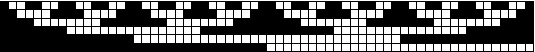
\includegraphics[width=4in]{BRGC6-cropped.pdf} 

\includegraphics[width=4in]{BCLX6-cropped.pdf} 

    \caption{Lexicographic (top), binary reflected Gray code (middle), and cool-lex (bottom) enumerations of 6-bit binary strings. Individual strings are read vertically from top to bottom.}
    \label{binary}
\end{figure}

\subsection{Cool-Lex Order}
% connect Gray code and cool-lex order
More recently, cool-lex order has introduced the idea of rotating sublists to enumerate languages.  Different versions of cool-lex order have been shown to enumerate several sets of combinatorial objects, including binary strings, fixed weight binary strings, Dyck words, and multiset permutations.  Cool-lex orders often lead to algorithms that are faster and simpler than standard lexicographic order.  For example, the ``multicool" package in R uses a loopless cool-lex algorithm to efficiently enumerate multiset permutations.   The package started using cool-lex order for multiset permutations in versoin 1.1 and as of version 1.12 has been downloaded nearly a million times \cite{multicool_2021}.
% minimal change order for stuff mentioned in 1.3
% say that the order leads to algorithms that are often simpler and faster than standard lexicographic order does
% for example, cite the multicool page and point out that (a) the package started with cool-lex for multiset permutations in version 1.1 and as of version 1.12 it has been downloaded nearly a million times
% https://www.rdocumentation.org/packages/multicool/versions/0.1-12
% maybe add something similar to Figure 1 for cool-lex of binary strings or combinations


% cool-lex for all binary strings
% conference: https://www.researchgate.net/publication/262153840_The_Coolest_Order_of_Binary_Strings
% journal: https://www.researchgate.net/publication/257376294_The_Coolest_Way_to_Generate_Binary_Strings

\subsection{Goals of this Thesis}

Cool-lex has been shown to provide a minimal-change cyclic ordering for the sets of fixed-weight binary strings, multiset permutations, binary and k-ary Dyck words, and other languages \cite{williams2009shift}. A common thread in the cool-lex algorithms for combinatorial generation is their focus on the \emph{first increase} of string, or the longest prefix of a string such that each successive symbol in the prefix is less than or equal to the previous symbol in the string.

This thesis will examine the use of cool-lex orders to enumerate other languages. Among these are Lukasiewicz, Motzkin, and Schröder paths, which are lattice paths that share similarities with Dyck paths. Shift Gray codes for enumerating these languages have been developed and are given in 1.3.

Dyck, Motzkin, Schröder, and Lukasiewicz paths all share bijections with various combinatorial objects. For example, Dyck paths of length $2n$ share a bijection with binary trees with $n$ nodes. Ruskey and Williams found that the cool-lex successor rule for enumerating Dyck words corresponded directly to a loopless successor rule for enumerating binary trees with a constant number of pointer changes \cite{ruskey2008generating}. This thesis will examine the efficiency of using cool-lex order to enumerate other sets of combinatorial objects in bijective correspondence with these languages.  

TODO: Describe new results of thesis?

